%%%%%%%%%%%%%%%%%%%%%%%%%%%%%%%%%%%%%%%%%%%%%%%%%%%%%%%%%%%%%%%%%%%%%%%%%%%%%%
%%Skeleton LaTeX file: double column format.
%%%%%%%%%%%%%%%%%%%%%%%%%%%%%%%%%%%%%%%%%%%%%%%%%%%%%%%%%%%%
%%REMEMBER THAT THERE IS AN EIGHT PAGE SIZE RESTRICTION
%%%%%%%%%%%%%%%%%%%%%%%%%%%%%%%%%%%%%%%%%%%%%%%%%%%%%%%%%%%%

%%% Sample file for ME Project Papers for Evaluation by Supervisor and Reader

\documentclass[]{article}

\setlength{\topmargin}{ 0.25in}
\setlength{\columnsep}{2.0pc}
\setlength{\headheight}{0.0in}
\setlength{\headsep}{0.0in}
\setlength{\oddsidemargin}{-.19in}
\setlength{\parindent}{1pc}
\textheight 8.75in
\textwidth 6.8in

\usepackage{multicol}
\usepackage{graphics}
\usepackage{url}
\usepackage[utf8]{inputenc}
\usepackage{etoolbox}

\usepackage{color,float}
\usepackage{boxedminipage}
\usepackage{epsfig} 
\usepackage{amsmath}
\usepackage{amssymb}
\usepackage{amsfonts}
\usepackage{comment}
\usepackage{tikz}
\usetikzlibrary{patterns}
\usepackage{subfig}
\DeclareCaptionType{copyrightbox}
\usepackage{algorithm}
\usepackage{algorithmic}
\usepackage{eqparbox}
\usepackage{times}

\newenvironment{Figure}
  {\par\medskip\noindent\minipage{\linewidth}}
  {\endminipage\par\medskip}

\bibliographystyle{unsrt}

\title{\large \bf On Demand Data Generation at Big Data Scale}
\author{Raghav Sood \\ Computer Science and Automation \\ Indian Institute of Science Bangalore \\ raghav@dsl.serc.iisc.ernet.in}

\date{October 18, 2016}

\begin{document}

    \maketitle
    \begin{center}
        Mid-term ME Project Report
    \end{center}
        \vskip 12pt
	
	\begin{abstract}
		OLAP engines are used widely in large data warehousing environments for Business Intelligence and Data Mining. 
		For performance testing these engines, the engine vendors commonly use synthetically generated datasets. 
		TPC-DS \cite{tpcds} is an industry-standard synthetic benchmark widely used for evaluating big data systems, but with its fixed schema and value distributions it represents only one particular data scenario. 
		Whereas a realworld client's scenario may be totally different. 
		It is because the schema changes and depending on the application, the value distributions greatly vary. 
		These characteristics of underlying data have a huge impact on execution of queries. 
		Thus engine's performance on TPC-DS may not be a good indicator of its performance on a particular client application.

		We are working on a data generation approach which takes as input the data characteristics of a given source database and generates synthetic data bearing similar characteristics. 
		Other challenges in large scale synthetic data generation are the space and time overheads involved in storing and indexing generated data. 
		This makes the existing technique- \cite{arasu} simply impractical at big data scale. 
		Our approach aims to mitigate these space and time overheads as it generates data \textit{on demand} i.e., instead of flushing generated data to any storage systems we plan to plug directly into the engine and supply synthetic tuples on-the-fly. 
		Our approach gives the ability to mimic a client's data scenario at vendor's development site which will be very useful for performance testing.
		It also gives the ability to mimic scaled up versions of existing data making it highly helpful in analyzing performance in futuristic environments. 
	\end{abstract}	
	
	\hfill
	
	\begin{multicols}{2}
	\section{Introduction}
		A database engine has broadly two components- the \textit{query optimizer} aka. planner and the \textit{executor}.
		A query is processed in two phases. 
		Compile-time processing is where given a query the optimizer comes up with an optimal plan. 
		Thereafter, at execution-time, the executor runs the given plan and produces results.
		Therefore, testing of database engine can be categorized into \textit{compile-time testing} and \textit{execution-time testing}.
		And effective testing is predicated on the ability to easily construct alternative scenarios with regard to the database contents \cite{codd}. 
		Our work is concerned with constructing particular scenarios in data which can be used for performance testing the executor.  
		
		The already available synthetic benchmarks like TPC-DS \cite{tpcds} are widely used to carry out performance tests in big data systems. 
		But such a benchmark represents only a particular data scenario. 
		The corresponding generator provided by TPC offers an option to generate various scaled versions of the benchmark.
		But the schema remains same and distribution of values in the generated data is not configurable.
		Also the TPC provided generator offers no option to manipulate data correlation across columns of same or multiple relations. 
		This is because of the fundamental reason that allowing such an option defeats the benchmark's purpose of objective and verifiable evaluation of systems. 
		Unfortunately, it makes these benchmarks far from various realistic customer scenarios to which a database vendor serves. 
		And hence engine's performance on TPC-DS may not be a good indicator of its performance on a particular client application.
		However, often using these benchmarks are the only possibility, as customer data and workloads are hard to obtain, due to their sensitive nature and moreover they are usually very large which makes transmission over the network hard if not impossible \cite{rsgen}.
		This may end up with unidentified performance bugs getting deployed. 
		\\ \\
                \textbf{Organisation: } In Section 2 we present our work in comparision to the related works in the field. 
		Section 3 includes the applications of our work. 
		Preliminaries are covered in Section 4. 
		Section 5 describes the problem statement formally and Section 6 describes our contributions. 
		Section 7 contains for reference additional details about select parts of our approach. 
		Findings from our preliminary experiments are in Section 8. 

	\section{Related Work}
		Related work \cite{arasu} has proposed generating \textit{workload-aware} datasets. 
		It captures the data characteristics of source database as a set of \textit{cardinality constraints}. 
		These constraints are then solved with the help of constraint solvers. 
		However, another related work RSGen \cite{rsgen} notes that this does not scale well to the amounts of data typically present in a customer dataset. 
		RSGen \cite{rsgen} is about generating data by \textit{reversing metadata statistics}. 
		This techniques scales linearly with the size of the database and works well in terms of recovering the metadata statistics and also in terms of volumetric similarity of \texttt{count} queries on single columns.
		However, the work accepts that data generated by their technique shows discrepencies for queries which go beyond the simple independent range queries. 
		In short, data generated by RSGen works for analyzing the behavior of query optimizer since it has fundamentally the same metadata characteristics. 
		But this data cannot be used to analyze the performance of executor because execution of a query depends highly on the \textit{fine-grained data characteristics}. 
		By fine-grained data characteristics we mean the operator level volumetric processing at each intermediate stage of a query plan. 
		
		We are working on a scalable approach to synthetically generate a database instance which has the same fine-grained data characteristics as the source database. 

		Our approach captures the desired data characteristics in a natural, expressive and declarative manner called \textit{cardinality constraints}. 
		Cardinality constraints were first introduced by \cite{arasu} and were also used in its followup work \cite{datasynth}. 
		In \cite{datasynth} the user can provide cardinality constraints manually by specifying a query expression and cardinality through a visual interface. 
		This becomes tedious and error-prone for large systems. 
		In our experiments we have found that to capture the data characteristics which ensure same behaviour of generated data on just 7 of the TPC-DS queries, one will have to enumerate 43 cardinality constraints. 
		We have implemented an automated technique to infer these constraints from a query plan. 		

		The workload for any database client application usually consists of a fixed set of queries. 
		And on an existing client database, running the \texttt{explain analyze} \cite{ea} command (in case of PostgreSQL or its equivalent command in case of other engines) for workload queries gives the output cardinalities of all intermediate operators as witnessed during the course of execution of that query. 
		Starting PostgreSQL version 9.0, this command outputs in program readable formats (xml/json/yml) which makes it very easy to capture the fine-grained data characteristics as cardinality constraints. 
		Thus we were able to programatically infer the constraints from output cardinality of intermediate operators appearing in query plans.
		Also we programatically infer the \textit{referential integrity constraints} from the schema. 
		A referential integrity constraint enforces that in our generated data, each synthetic value we use in a foreign-key column also exists in the corresponding primary key column. 

		We then formulate these cardinality and referential integrity constraints as a \textit{Linear Program (LP)}\footnote{The LP in our case has no optimization object, rather all what we are interested in is to get a feasible solution for the LP constraints. }.
		But we find it is NOT scalable and we are exploring some matrix based formulations of the problem. 
		The LP solution can be represented as a \textit{database summary} which we believe will be in order of megabytes while the original database could be in terabytes to petabytes.
		This database summary will be next used as a seed to our on-demand synthetic tuple generator. 
		
	\section{Applications}
		Once above components are in place, we will be able to synthetically generate a \textit{virtual} database instance, which for the predefined workload queries, behaves similar to the client's database.
		Note that the similarity here is in \textit{volumetric terms} i.e., getting the same number of output tuples at each intermediate operator in the query plan. 
                
		This ability to mimic a client's data scenario at the database vendor's development site will be very useful for database engine testing.
		Also the approach serves as a \textit{data masking} technique. 
		Client organisations which outsource the testing of their database application find it difficult to share the dataset alongwith primarily because of two reasons- 
		(a) privacy concerns 
		(b) size of the dataset being huge (terabytes to petabytes). 
		These organisations will now have to share just the workload queries and the query plans (more precisely, the ALQPs which are defined in Section 4.1). 
		These are typically in a few hundred megabytes and using our approach, the tester will be able to generate the synthetic data at his site. 
		Thus the cost and time of network transmission is forgone and also the dataset which tester now gets is, in a way, a masked version of original dataset. 
		
		As found in our industry interactions with both HP Enterprise (a database vendor) and TCS (a database testing service provider) our work will be very useful to them. 
		Also it was pointed out to us that, in most cases client organisations are fine with sharing their database schema and workload query templates but they are unwilling to share the parameterized workload queries. 
		In such cases our approach is still applicable as all the workload queries and the query plans can be encrypted with any order-preserving encryption technique. 
		The approach also gives the ability to mimic scaled versions of existing data making it highly helpful in analyzing performance in futuristic environments.
		
	\section{Preliminaries}
	        \subsection{Annotated Logical Query Plan (ALQP)}
		A logical query plan is an extended relational algebra tree. 
		It gives the set of operations involved in executing a query as per their sequence. 
		An ALQP is a logical query plan which in addition also gives input and output cardinalities for each operator in the tree. 
		The input cardinality specifies the number of tuples that reach the operator and the output cardinality gives the number of tuples that leave the operator. 
		An example SQL query with its corresponding ALQP is shown in Figure 1. 
		
		\subsection{Cardinality Constraints}
		Assuming that $\mathcal{R}_1, ... , \mathcal{R}_l$ are the set of relations in the database, each operator in the ALQP corresponds to a cardinality constraint that can be written in the following form:
			\begin{equation}
				| \sigma_\mathcal{P} (\mathcal{R}_{i_1} \bowtie ... \bowtie \mathcal{R}_{i_p}) | = k
			\end{equation}
		where $\mathcal{P}$ is a selection predicate, and $k$ is a non-negative integer.
		For example, the constraints that can be derived from the ALQP shown in Figure 1 are:
			\begin{align}
				|W| & = 7197559 \nonumber \\
				|D| & = 73066 \nonumber \\
				|I| & = 102006 \nonumber \\
				|\sigma_{d\_month\_seq >= 1211}(D)| & = 36192 \nonumber \\
				|\sigma_{d\_month\_seq >= 1211}(W \bowtie D)| & = 3131870 \\
				|\sigma_{d\_month\_seq >= 1211}(W \bowtie D \bowtie I)| & = 3131870
			\end{align}

		{
		\begin{tabular}{ |p{0.8\linewidth}| }
			\hline
			select * from \\ 
			web\_sales W, date\_dim D, item I \\ 
			where D.d\_month\_seq $>$= 1211 \\ 
			and W.ws\_sold\_date\_sk = D.d\_date\_sk \\ 
			and W.ws\_item\_sk = I.i\_item\_sk \\
			\hline
			\begin{Figure}
				\centering
				
\includegraphics[width=0.8\linewidth]{figures/alqp1.png}
				\label{fig:alqp1}
			\end{Figure} \\
			\hline
		\end{tabular}
		\captionof{figure}{An example query with corresponding ALQP}
		}
		
	\section{Problem Statement}
			\begin{tabular}{ |p{0.9\linewidth}| }
			\hline
				Given a database schema $\mathcal{S}$ and a set of ALQPs  $\mathcal{A}$, generate a database instance that conforms to $\mathcal{S}$ and satisfies closely all the cardinality constraints ($\mathcal{C}_1, \mathcal{C}_2, ... , \mathcal{C}_m$) generated from $\mathcal{A}$. \\
			\hline
			\end{tabular}
			\\ \\ 
		Schema $\mathcal{S}$ includes- (a) list of names of all the tables (b) list of names of columns in each table (c) list of foreign keys and their corresponding primary keys. 
		Set of ALQPs $\mathcal{A}$ has info on number of tuples outputed by each operator in the query plans corresponding to a fixed set of user queries. 

		The decision version\footnote{In the decision version of the problem, the output is YES if there exists a database instance that satisfies all the constraints and NO otherwise.} of this problem is \textit{NEXP-complete} \cite{arasu}.
		But in our case, since the constraints are indeed derived from the ALQPs found on the source database, we already know that output of decision version is YES. 
		
	\section{Our Contributions}
		We are working on implementing \cite{arasu, datasynth} with following additonal goals: 
		\begin{itemize}
			\item Remove the manual step of feeding in as input the cardinality constraints as it is tedius and error prone. 
			\item Study scalability of the constraint solving technique presented in their work and improve upon it if possible. 
			\item Make the data generation \textit{on demand} i.e., instead of flushing generated data to any storage systems we plan to plug directly into the engine and supply synthetic tuples on-the-fly.
		\end{itemize}
		The above goals are partly achieved while we are working on the rest. 
		
		\subsection{Current Status}
		\begin{itemize}
			\item {\bf Parser:}
			The purpose of parser is to take $\mathcal{A}$ as input and give the set of cardinality constraints as described in Section 4.2
			We found that starting PostgreSQL version 9.0, the \texttt{explain analyze} command outputs in \textit{json} format which is program readable.
			We have implemented a code module in java to parse this json text.
			Thus we were able to programatically infer the constraints from output cardinalities of intermediate operators appearing in query plans.
			This removes the tedious and error prone manual step of framing the input in \cite{datasynth}. 

            \item {\bf View Generator:}
            This component takes the database schema as input and creates a view $\mathcal{V}_{i}$ corresponding to every relation $\mathcal{R}_{i}$.
	    It is an implementation of the concept of a view and the view generation strategy of \cite{arasu}. 
            In short, creation of views help us to get rid of the join expressions in the constraints. 
            Each constraint may involve multiple relations being joined together. 
            By view generation we will be able to re-write it as a constraint over a single view.
            More details are in Section 7.1.

            \item {\bf LP Formulator:}
            This component uses the views given by the view generator to re-write the cardinality constraints given by the parser.
            Further, an LP is created for each view. This is done by converting each constraint (on that view) to a corresponding equation.
            Once this is done, the system of equations is passed on to the LP solver.
            More details are in Section 7.2.

		\end{itemize}

		\subsection{In Progress}			
		\begin{itemize}
			\item {\bf LP Solver:}
            This component takes the system of equations and gives one of the feasible solutions. 
            \footnote{The system of equations can have infinite solutions.
            The solution corresponding to the original database instance might differ from the solution we get here. But, both the solutions would satisfy all the cardinality constraints.}.
            We use the GNU Linear Programming Kit (GLPK) \cite{glpk} for solving the LP.
            Currently we are limiting to a set of maximum 7 queries as the number of variables in the LP grows exponentially with the queries.

            \item {\bf Relation Generator:}
            This component takes the solution given by the LP solver and represents it in a concise format which we call the \textit{database summary} which we believe will be in order of megabytes while the original database could be in terabytes to petabytes.
        This database summary will be next used as a seed to our on-demand synthetic tuple generator.
            
            \item {\bf Tuple Generator:}
            The database summary that we obtain from the relations generator serve as the seeds to the tuple generator. 
			We plan to embed this generator in the code of Postgres by which we will be able to supply tuples on demand.
			This mitigates the space and time overheads of flushing the generated data to any physical storage and indexing it. 
        \end{itemize}
	
		Figure 2 provides an overview of the architecture\footnote{The architecture and the division of functionality in each module was designed by my lab senior, Anupam Sanghi, 2015-2016. } of the data generator we working on.
        \begin{Figure}
                \centering
                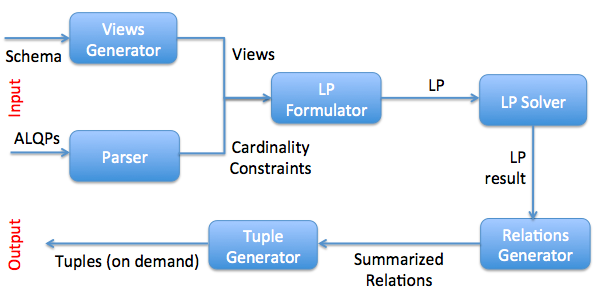
\includegraphics[width=\linewidth]{figures/architecture.png}
                \captionof{figure}{Architecture of the Data Generator}
                \label{fig:Architecture}
        \end{Figure}

        \subsection{Future Work}
        \begin{itemize}
		    \item {\bf Scalability:}
		    It was noted by \cite{rsgen} that the constraint solving strategy proposed in \cite{arasu, datasynth} does NOT scale well. 
			It is understandable as it uses LP solvers and the number of LP variables may increase exponentially with the number of queries. 
			We will be exploring two directions to address scalability- 
			(a) using a matrix based formulation of the problem and solving a linear system of the form- $Ax = b$  
			(b) relax the cardinality constraints to accept approximate solutions. 

			\item {\bf Projection Operator:}
			The support provided by \cite{arasu, datasynth} for \textit{project operator} is limited to only single columns. 
			A direction to explore would be to devise an algorithm which supports generic project operator. 
        \end{itemize}

	\section{More Details on Current Work}
	
		\subsection{View Generator}
			As discussed earlier, the purpose of this component is to simplify the constraints such that we can replace all the join expressions by a single view. 
			For this we need to construct a view $\mathcal{V}_{i}$ corresponding to each relation $\mathcal{R}_{i}$. 
			A view $\mathcal{V}_{i}$ can be considered as a set of non-key attributes that are present in either $\mathcal{R}_{i}$ or in any other relation on which $\mathcal{R}_{i}$ depends. 
			The dependencies between relation can be seen from the {\em dependency graph}.
			
			{\bf Dependency Graph:} 
			In a dependency graph, we create a node for every relation. 
			A directed edge from a node $\mathcal{R}_{i}$ to $\mathcal{R}_{j}$ is added, if $\mathcal{R}_{i}$ contains a {\em foreign-key} referencing $\mathcal{R}_{j}$.
			Now, a relation $\mathcal{R}_{i}$ is said to be dependent on relation $\mathcal{R}_{j}$ if there exists a path from $\mathcal{R}_{i}$ to $\mathcal{R}_{j}$ in the dependency graph.
		
			For example, consider a database having the following four relations:
			\begin{align*}
				& Catalog\_sales (\underline {PK_{1}}, FK_{C}, FK_{D}, cs\_sales\_price) \\
				& Customer (\underline {PK_{2}}, FK_{CA}) \\
				& Date\_dim (\underline {PK_{3}}, d\_qoy, d\_year) \\
				& Customer\_address (\underline {PK_{4}}, ca\_state)
			\end{align*}
			
			Here, $PK_{1}$, $PK_{2}$, $PK_{3}$, $PK_{4}$ are the primary keys of the respective relations. 
			$FK_{C}$ references to $Customer$, $FK_{D}$ references to $Date\_dim$ and $FK_{CA}$ references to $Customer\_address$. 
			Therefore, the dependency graph would be as shown in Figure 3. 
			
			\begin{Figure}
				\centering
				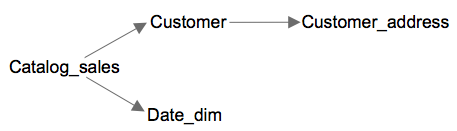
\includegraphics[width=\linewidth]{figures/schema_dig.png}
				\captionof{figure}{Dependency Graph}
				\label{fig:dependency-graph}
			\end{Figure}
			
			By traversing the dependency graph in reverse topological sort order, a view corresponding to each relation is generated. The generated views for the above example are: 
			\begin{align*}
				& Catalog\_sales' (ca\_state, d\_qoy, d\_year, cs\_sales\_price) \\
				& Customer' (ca\_state) \\
				& Date\_dim' (d\_qoy, d\_year) \\
				& Customer\_address' (ca\_state)
			\end{align*}
	
		\subsection{LP Formulator}
			The LP Formulator receives the set of constraints from the parser and the set of views from the view generator. 
			The first task it does is to re-write the constraints by replacing the join expressions with appropriate views. 
			Say we have a constraint having join: $\mathcal{R}_{i} \bowtie \mathcal{R}_{k}$. 
			We assume that all joins are of primary key-foreign key type, hence one of these is a dependent relation. 
			Say $\mathcal{R}_{i}$ depends on $\mathcal{R}_{k}$. 
			In such a case, we shall replace the expression $\mathcal{R}_{i} \bowtie \mathcal{R}_{k}$ with $\mathcal{V}_{i}$. 
			Because of the way we constructed the views, it is easy to see that we can apply the predicates that were there on  $\mathcal{R}_{i} \bowtie \mathcal{R}_{k}$ to $\mathcal{V}_{i}$. 
			Likewise, all the join expressions can be expressed in terms of a single view respectively.
			
			Continuing on the example shown in Figure 1, considering that the dependency graph is rooted at node $W$ having two children $D$ and $I$, the cardinality constraints in equation 2 and 3 can be rewritten as:
			\begin{align*}
				& |\sigma_{d\_month\_seq >= 1211}(W')| = 3131870 \\
				& |\sigma_{d\_month\_seq >= 1211}(W')| = 3131870
			\end{align*}
			where $W'$ represents the view corresponding to $W$. 
			The duplicate constraint can be ignored as it doesn't add any new information.
			
			Now we solve for each view separately. 
			We need to formulate an LP for $\mathcal{V}$. 
			Let's find the set of constraints imposed on $\mathcal{V}$. 
			A constraint $\mathcal{C}_{j}$ on $\mathcal{V}$ will be of the following form:
			\begin{equation*}
				| \sigma_{\mathcal{P}_{j}} (\mathcal{V})| = k_{j}
			\end{equation*}
			Say we are given a set of $m$ constraints that $\mathcal{V}$ satisfies. 
			Each constraint $C_{j}$  $(1 \leq j \leq m)$ for simplicity can be expressed as: $<\mathcal{P}_{j}, k_{j}>$, which means that the number of tuples (rows) satisfying the predicate $\mathcal{P}_{j}$ is equal to $k_{j}$. 
			
			Let $A_{1}$, $A_{2}$,...,$A_{n}$ be the attributes we have in view $\mathcal{V}$. 
			Let the domain of an attribute $A_{i}$ be represented by $Dom(A_{i})$. 
			We assume that the domain of all the attributes is the set of positive integers. 
			For attributes with non-integral domains, we can map the values to integers. 
			This assumption is to simplify the analysis and can be removed easily.
			
			For every tuple $t \in Dom(A_{1}) \times Dom(A_{2})\times...\times Dom(A_{n})$, we create a variable $x_{t}$ to represent the number of copies of $t$ in $\mathcal{V}$. 
			Now, for each of the $m$ constraints $C_{j}$ $(1 \leq j \leq m)$, we create a linear equation:
			\begin{equation*}
				\sum_{t:P_{j}(t)=true} x_{t} = k_{j}
			\end{equation*}
			
			Also we add non-negativity constraints $x_{t} \geq 0$ $\forall t$ to the LP. 
			And as the solution of the LP need not be integral, we shall use the simple {\em rounding technique} on the solution. 
			
			Further, since the number of variables in the LP is proportional to the domain size, it can be huge. 
			Next is an optimisation proposed in \cite{arasu} to reduce the size of the LP. 
			\\ \\
			\textbf{Domain Decomposition: }
			A set $v^{i}$ is created for each attribute $A_{i}$. 
			Values in  $v^{i}$ are added according to the following: 
			
			We iterate over the constraints and if a constraint has
			\begin{itemize}
				\item $A_{i} >= a$ or $A_{i} < a$, then add $a$ in  $v^{i}$.
				\item $A_{i} > a$ or  $A_{i} <= a$, then add $a + 1$ in $v^{i}$.
				\item $A_{i} = a$, then add $a$ and $a+1$ both in $v^{i}$.
			\end{itemize}
			
			All the other constraints can be expressed as combinations of the above. 
			In addition, we also add $1$ (minimum value in domain) in $v^{i}$ if not already present. 
			Let  $v_{1}^{i}, v_{2}^{i},...,v_{l_{i}}^{i}$ represent the constants (in increasing order) in the set $v^{i}$. 
			Now we can divide the domain of an attribute $A_{i}$ into $l_{i}$ mutually exclusive and exhaustive intervals $I^{i}: [v_{q}^{i},v_{q+1}^{i})$ $(1 \leq q < l_{i}) \cup [v_{l_{i}}^{i},)$. 
			The semantics of the variables can now be modified such that we introduce a variable $x_{t'}$ for each interval combination $t' \in I^{1} \times I^{2} \times ... \times I^{n}$, to represent the number of tuples lying in the interval combination $t'$.
			
			Therefore, now for each constraint $C_{j}$ $(1 \leq j \leq m)$, the linear equation would be:
			\begin{equation*}
				\sum_{t':P_{j}(t')=true} x_{t'} = k_{j}
			\end{equation*}
			Here as well we will have the additional constraint of $x_{t'} \ge 0$ $\forall t'$.
			
			For example, let us see the LP formulation for relation $Catalog\_sales$ having following constraints:
			{\small
			\begin{align*}
				|CS| & = 14401261 \\
				|\sigma_{cs\_sales\_price > 150} (CS)| & = 734606 \\
				|\sigma_{cs\_sales\_price > 150 \wedge ca\_state = 1} (CS)| & = 13806
			\end{align*}
			}
			These constraints can be converted into the corresponding LP equations as follows:
			{\small
			\begin{align*}
				x_{[1,151)[1,2)} + x_{[1,151)[2,)} + x_{[151,)[1,2)} + x_{[151,)[2,)} & = 14401261	\\
				x_{[151,)[1,2)} + x_{[151,)[2,)} & = 734606 \\
				x_{[151,)[1,2)} & = 13806
			\end{align*}
			}
			Therefore, we can see that by applying this optimization, the number of variables are a function of the size of the sets $v^{i}$s instead of the domain size. 
			But, even after applying this optimization, the number of variables are exponential in the number of attributes. 
			
			
	\section{Experiments}
		For the preliminary experiments at this stage, we have the following setup:
		\begin{itemize}
			\item 100GB version of TPC-DS v2.3.0 \cite{tpcds} is taken as the source database for generation
			\item 7 of the TPC-DS queries numbered 3, 22, 42, 50, 52, 55, 62 are chosen for extracting cardinality constraints
			\item PostgreSQL v9.5.4 is the database engine
		\end{itemize}
		Each of the 7 queries is first ran with the \texttt{explain analyze (format=json) ... } command to get the query plans along with intermediate cardinality values. 
		The parser module then extracts out cardinality constraints from the json text. 
		We have some initial findings on the sizes of the LPs formulated.
		\\ \\
		{\scriptsize
                \begin{tabular}{ |p{0.2\linewidth}|p{0.1\linewidth}|p{0.2\linewidth}|p{0.2\linewidth}| }
                        \hline
                        TPC-DS Q\# & \# LPs & \# Vars in biggest LP & \# Constraints in biggest LP \\
                        \hline
                        Q3 & 3 & 9 & 4 \\
                        Q22 & 3 & 3 & 4 \\
                        Q42 & 3 & 27 & 4 \\
                        Q50 & 4 & 9 & 5 \\
                        Q52 & 3 & 27 & 4 \\
                        Q55 & 3 & 27 & 4 \\
                        Q62 & 3 & 3 & 6 \\
                        \hline
                        Set of all 7 queries & 10 & 1350 & 17 \\
                        \hline
                \end{tabular}
		\captionof{table}{LP sizes for various TPC-DS queries}
		}

	 	Note that each query can span accross multiple views and for each view an independent LP problem is formulated and solved.
	 	By biggest LP, we here mean the LP with maximum number of variables. 
		In Table 1 we report the number of LPs to be solved when each of the 7 queries was considered in isolation i.e., we extract cardinality constraints from the single query. 
		The solution to LPs in this case represents a synthesized database which given the same query will show the same volumetric behaviour at each level of the query plan. 
		The last row shows the case when all 7 queries were considered together. 
		The solution to LPs in this case represents a synthesized database which will show similar volumetric behaviour for all of the 7 queries. 
		\\ \\
		\textbf{Understandings from the experiments: }
			\begin{itemize}
                    		\item The size of LP blows up with just 7 queries. 
                    		\item When we take a few queries together, the LPs become highly underconstrained.
                    		\item LP solvers won't scale for real world scenarios which may have 50-100 queries. 
				\item The LPs in our case bear very \textit{special} properties:
			\begin{itemize}
                	\item It is a feasibility LP i.e., objective function is constant.
                	\item All variable have binary coefficients in the constraints. 
                	\item Other than the non-negativity constraints for each variable, all constraints are equality constraints. 
                	\item Each constraint equals a non-negative integral value. 
			\item It is known that LP is feasible i.e., it has atleast one solution (since it is formulated starting from an existing database). 
        	\end{itemize}
			The generic LP solvers won't exploit these special properties of our problem. 
			And hence we are looking for some matrix based solution which because of these properties may be much more efficient. 
		\end{itemize}


\begin{thebibliography}{7}
\bibitem{ea}
explain analyze PostgreSQL v9.5. \url{https://www.postgresql.org/docs/9.5/static/using-explain.html}, 2016.

\bibitem{glpk}
GLPK v4.60. \url{https://www.gnu.org/software/glpk/}, 2016.

\bibitem{tpcds}
TPC-DS v2.3.0. \url{http://www.tpc.org/tpcds}, 2016.

\bibitem{arasu}
Arvind Arasu, Raghav Kaushik and Jian Li. Data generation using declarative constraints. SIGMOD, 2011.

\bibitem{datasynth}
Arvind Arasu, Raghav Kaushik and Jian Li. Datasynth: Generating synthetic data using declarative constraints. PVLDB, 2011.

\bibitem{rsgen}
Entong Shen and Lyublena Antova. Reversing statistics for scalable test databases generation. DBTest, 2013.

\bibitem{codd}
Rakshit S. Trivedi, I. Nilavalagan and Jayant R. Haritsa. CODD:  COnstructing Dataless Databases. DBTest, 2012.

\end{thebibliography}
	
\end{multicols}
\end{document}
